\documentclass[handout]{beamer}
\usepackage[utf8]{inputenc}
\usepackage[T2A]{fontenc}
\usepackage[english]{babel}
\usepackage{graphicx}
\usetheme{Warsaw}
\usecolortheme{wolverine}

\usepackage{listings}
\usepackage{color}
\usepackage{amsmath}
\usepackage{changepage}

\definecolor{dkgreen}{rgb}{0,0.6,0}
\definecolor{gray}{rgb}{0.5,0.5,0.5}
\definecolor{mauve}{rgb}{0.58,0,0.82}

\lstdefinelanguage{Haskell}%
  {otherkeywords={},%
   morekeywords={as,abstype,if,then,else,case,class,data,default,deriving,%
      hiding,if,in,infix,infixl,infixr,import,instance,let,module,%
      newtype,of,qualified,type,where,do,AbsoluteSeek,AppendMode,%
      Array,BlockBuffering,Bool,BufferMode,Char,Complex,Double,Either,%
      FilePath,Float,Int,Word,Integer,Natural,IO,IOError,Ix,LineBuffering,Maybe,%
      Ordering,NoBuffering,ReadMode,ReadWriteMode,ReadS,RelativeSeek,%
      SeekFromEnd,SeekMode,ShowS,StdGen,String,Void,Bounded,Enum,Eq,%
      Eval,ExitCode,exitFailure,exitSuccess,Floating,Fractional,%
      Functor,Handle,HandlePosn,IOMode,Integral,List,Monad,MonadPlus,%
      MonadZero,Num,Numeric,Ord,Random,RandomGen,Ratio,Rational,Read,%
      Real,RealFloat,RealFrac,Show,System,Prelude,EQ,False,GT,Just,%
      Left,LT,Nothing,Right,WriteMode,True,abs,accum,accumArray,%
      accumulate,acos,acosh,all,and,any,ap,appendFile,applyM,%
      approxRational,array,asTypeOf,asin,asinh,assocs,atan,atan2,atanh,%
      bounds,bracket,bracket_,break,catch,catMaybes,ceiling,chr,cis,%
      compare,concat,concatMap,conjugate,const,cos,cosh,curry,cycle,%
      decodeFloat,delete,deleteBy,deleteFirstsBy,denominator,%
      digitToInt,div,divMod,drop,dropWhile,either,elem,elems,elemIndex,%
      elemIndices,encodeFloat,enumFrom,enumFromThen,enumFromThenTo,%
      enumFromTo,error,even,exitFailure,exitWith,fail,%
      filter,filterM,find,findIndex,findIndices,flip,floatDigits,%
      floatRadix,floatRange,floatToDigits,floor,foldl,foldM,foldl1,%
      foldr,foldr1,fromDouble,fromEnum,fromInt,fromInteger,%
      toInteger,fromJust,fromMaybe,fromRat,fromRational,%
      fromRealFrac,fst,gcd,genericLength,genericTake,genericDrop,%
      genericSplitAt,genericIndex,genericReplicate,getArgs,getChar,%
      getContents,getEnv,getLine,getProgName,getStdGen,getStdRandom,%
      group,groupBy,guard,hClose,hFileSize,hFlush,hGetBuffering,%
      hGetChar,hGetContents,hGetLine,hGetPosn,hIsClosed,hIsEOF,hIsOpen,%
      hIsReadable,hIsSeekable,hIsWritable,hLookAhead,hPutChar,hPutStr,%
      hPutStrLn,hPrint,hReady,hSeek,hSetBuffering,hSetPosn,head,%
      hugsIsEOF,hugsHIsEOF,hugsIsSearchErr,hugsIsNameErr,%
      hugsIsWriteErr,id,ioError,imagPart,indices,init,inits,%
      inRange,insert,insertBy,interact,intersect,intersectBy,%
      intersperse,intToDigit,ioeGetErrorString,ioeGetFileName,%
      ioeGetHandle,isAlreadyExistsError,isAlreadyInUseError,isAlpha,%
      isAlphaNum,isAscii,isControl,isDenormalized,isDoesNotExistError,%
      isDigit,isEOF,isEOFError,isFullError,isHexDigit,isIEEE,%
      isIllegalOperation,isInfinite,isJust,isLower,isNaN,%
      isNegativeZero,isNothing,isOctDigit,isPermissionError,isPrefixOf,%
      isPrint,isSpace,isSuffixOf,isUpper,isUserError,iterate,ixmap,%
      join,last,lcm,length,lex,lexDigits,lexLitChar,liftM,liftM2,%
      liftM3,liftM4,liftM5,lines,listArray,listToMaybe,log,logBase,%
      lookup,magnitude,makePolar,map,mapAccumL,mapAccumR,mapAndUnzipM,%
      mapM,mapM_,mapMaybe,max,maxBound,maximum,maximumBy,maybe,%
      maybeToList,min,minBound,minimum,minimumBy,mkPolar,mkStdGen,%
      mplus,mod,msum,mzero,negate,next,newStdGen,not,notElem,nub,nubBy,%
      null,numerator,odd,openFile,or,ord,otherwise,partition,phase,pi,%
      polar,pred,print,product,properFraction,putChar,putStr,putStrLn,%
      quot,quotRem,random,randomIO,randomR,randomRIO,randomRs,randoms,%
      rangeSize,read,readDec,readFile,readFloat,readHex,readInt,readIO,%
      readList,readLitChar,readLn,readParen,readOct,readSigned,reads,%
      readsPrec,realPart,realToFrac,recip,rem,repeat,replicate,return,%
      reverse,round,scaleFloat,scanl,scanl1,scanr,scanr1,seq,sequence,%
      sequence_,setStdGen,show,showChar,showEFloat,showFFloat,%
      showFloat,showGFloat,showInt,showList,showLitChar,showParen,%
      showSigned,showString,shows,showsPrec,significand,signum,sin,%
      sinh,snd,sort,sortBy,span,split,splitAt,sqrt,stderr,stdin,stdout,%
      strict,subtract,succ,sum,system,tail,tails,take,takeWhile,tan,%
      tanh,toEnum,toInt,toInteger,toLower,toRational,toUpper,transpose,%
      truncate,try,uncurry,undefined,unfoldr,union,unionBy,unless,%
      unlines,until,unwords,unzip,unzip3,unzip4,unzip5,unzip6,unzip7,%
      userError,when,words,writeFile,zero,zip,zip3,zip4,zip5,zip6,zip7,%
      zipWith,zipWithM,zipWithM_,zipWith3,zipWith4,zipWith5,zipWith6,%
      zipWith7},%
   sensitive,%
   morecomment=[l]--,%
   morecomment=[n]{\{-}{-\}},%
   morestring=[b]"%
  }[keywords,comments,strings]%

\lstset{
  language=Haskell,
  showstringspaces=false,
  columns=flexible,
  keepspaces=true,
  basicstyle={\ttfamily},
  numbers=none,
  numberstyle=\tiny\color{gray},
  keywordstyle=\color{blue},
  commentstyle=\color{dkgreen},
  stringstyle=\color{mauve}
}

\title[Dependent bookkeeping]{Dependent types in Haskell and bookkeeping}
\author[Andrew Lelechenko]{Andrew Lelechenko \\ \texttt{1@dxdy.ru}}
\date{F(café), Kiev, 20.06.2017}

\begin{document}

\begin{frame}
	\titlepage
\end{frame}

\begin{frame}[fragile]{Why not Haskell?}

Paul Hudak, John Hughes, Simon Peyton Jones, Philip Wadler,
  {\em A~History of Haskell: Being Lazy With Class,} HOPL-III, 2007.

\bigskip

\begin{itemize}\itemsep2ex
\item Haskell is lazy.
\item Haskell is pure.
\item Haskell has type classes.
\end{itemize}

\bigskip

\centerline{\Huge\bf Do you care?}

\end{frame}

\begin{frame}[fragile]{The Languages We Call Haskell © Don Stewart, 2010}

\vspace{-1.5ex}

\begin{figure}[H]
\centering
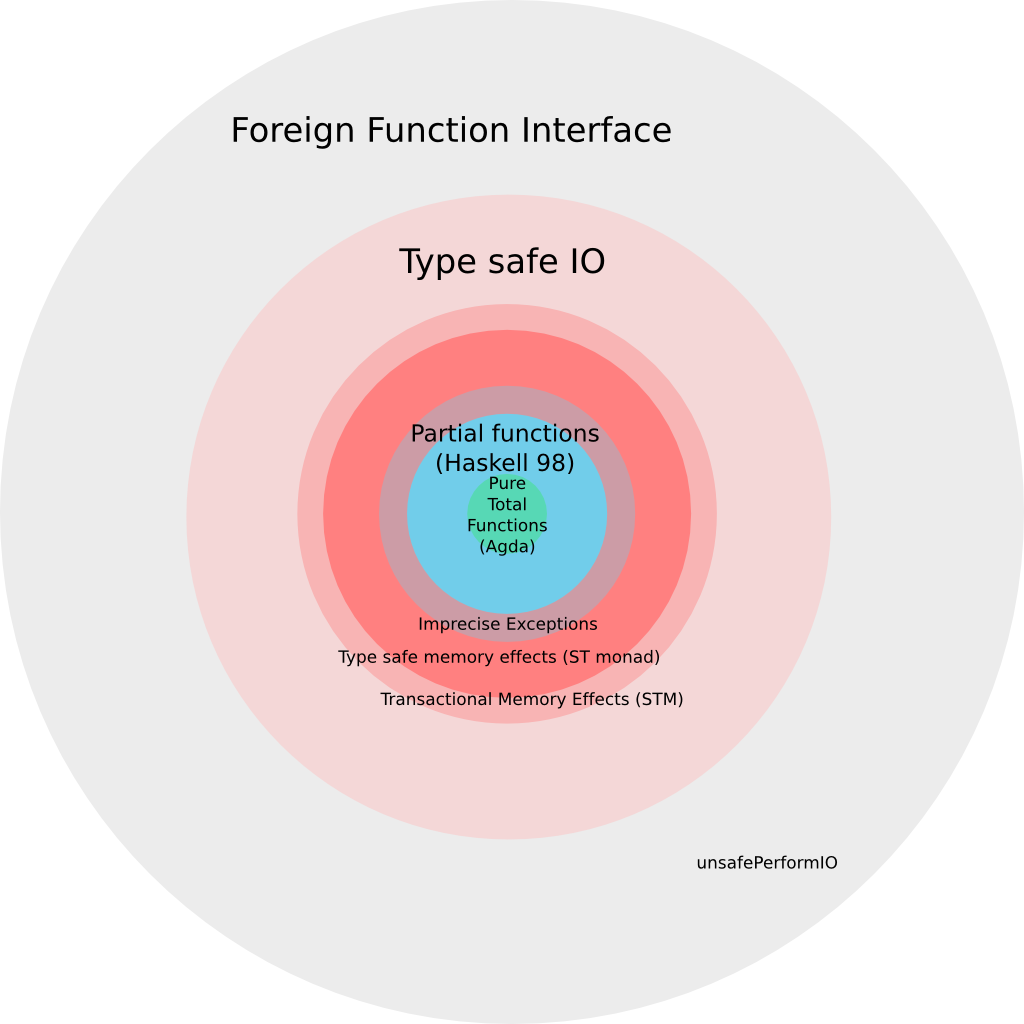
\includegraphics[width=0.9\textwidth]{circles.png}
\end{figure}

\end{frame}

\begin{frame}[fragile]{So why Haskell?}

\begin{itemize}

\item Haskell is a practical language. The number of active GitHub repos is only 25x less than in Java (http://githut.info).

\item Haskell is easy to read, easy to reason about and easy to refactor.
  It~is not so easy to write, however.

\item Haskell offers ample performance for most applications and great options for parrallel/concurrent computations.
  See L.~Petersen, T.~A.~Anderson, H. Liu, N. Glew, {\em Measuring the~Haskell Gap,} IFL, 2013.

\item Haskell encourages advanced type discipline, allowing to specify and check invariants in compile time.
  {\em Very important:} types are not about `do not confuse {\tt string} with {\tt int}', types are propositions.

\end{itemize}

\end{frame}

\begin{frame}[fragile]{The Haskell Pyramid © Lucas Di Cioccio, 2017}

\begin{figure}[H]
\centering
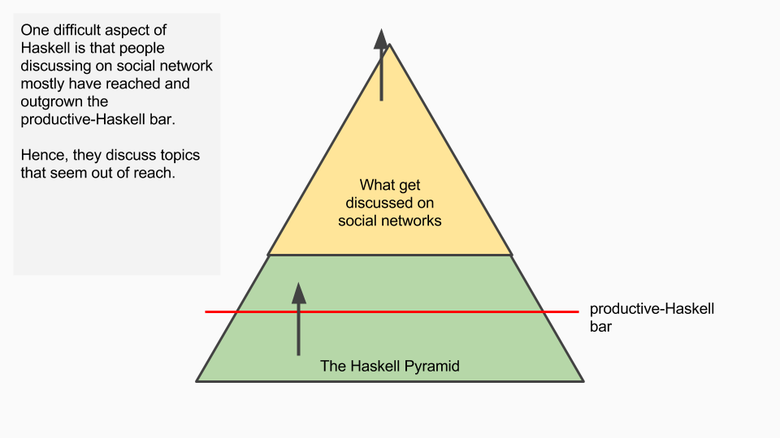
\includegraphics[width=1.1\textwidth]{pyramid.png}
\end{figure}

\end{frame}

\begin{frame}[fragile]{Rounding is tricky}

\begin{itemize}

\item There are many modes of rounding: CEILING / FLOOR, UP~/~DOWN, HALF\_UP / HALF\_DOWN, HALF\_EVEN.
  Further we assume HALF\_EVEN everywhere, which rounds towards the `nearest neighbor' unless both neighbors are equidistant,
  in which case, round towards the even neighbor.

\item Rounding does not distribute over arithmetic operations:

\end{itemize}

\begin{lstlisting}
round(x, prec) + round(y, prec) /= round (x + y, prec)
\end{lstlisting}

\begin{lstlisting}
round(1/3, 2) + round(1/3, 2) = 0.66
round(1/3 + 1/3, 2) = 0.67
\end{lstlisting}

\begin{itemize}
\item Roundings with different precisions do not commute:
\end{itemize}

\begin{lstlisting}
round(round(x, pr1), pr2) /= round(round(x, pr2), pr1)
\end{lstlisting}

\begin{lstlisting}
round(round(1.49, 1), 0) = round(1.50, 0) = 2.00
round(round(1.49, 0), 1) = round(1.00, 1) = 1.00
\end{lstlisting}

\end{frame}

\begin{frame}[fragile]{{\tt Decimal} reinvented}

Precision can be treated as a negative exponent.

\begin{lstlisting}
data Decimal = Decimal
  { exp :: Integer, mantissa :: Integer }

instance Show Decimal where
  show d = show (fromInteger (mantissa d) /
                    10 ^ exp d)

foo = Decimal 2 12345 :: Decimal
-- show foo = "123.45"
\end{lstlisting}

\begin{lstlisting}
instance Num Decimal where
  (Decimal exp1 mant1) + (Decimal exp2 mant2) = ?
\end{lstlisting}

How can we implement arithmetic operations on decimals with mixed exponents?

\end{frame}

\begin{frame}[fragile]{Addition of {\tt Decimal}s}

\begin{itemize}

\item Cast both numbers to the highest precision, then add:

    1.2 + 1.23 = 1.20 + 1.23 = 2.43

    Decimal 1 12 + Decimal 2 123 = Decimal 2 243

    This is simply unlawful.

\item Cast both numbers to the lowest precision, then add:

    1.2 + 1.23 = 1.2 + 1.2 = 2.4

    Decimal 1 12 + Decimal 2 123 = Decimal 1 24

    Precision decreases silently. And most of the time this is an error.

\item Throw an error, if exponents are not equal.
    So much pure and strict, but such addition does not fit into type class {\tt Num}.

\end{itemize}

\end{frame}

\begin{frame}[fragile]{{\tt Decimal} re-reinvented}

Goal: mismatch of precisions should be ruled out by construction.

Compare
\begin{lstlisting}
data Decimal =
  Decimal { exp :: Integer, mantissa :: Integer }
\end{lstlisting}
vs.
\begin{lstlisting}
newtype Decimal ( exp :: Nat ) =
  Decimal { mantissa :: Integer }
\end{lstlisting}

E. g.,
\begin{lstlisting}
foo :: Decimal 2
foo = Decimal 12345
-- means 123.45, previously Decimal 2 12345

bar :: Decimal 3
bar = Decimal 12345
-- means 12.345, previously Decimal 3 12345
\end{lstlisting}

\end{frame}

\begin{frame}[fragile]{Why type-level {\tt Nat} matters?}

\begin{itemize}

\item (+) :: Decimal $\to$ Decimal $\to$ Decimal

    This type signature is a proposition: if you give me one Decimal,
    and then another Decimal, I'll return some other Decimal. Rather weak contract.

\item (+) :: Decimal exp $\to$ Decimal exp $\to$ Decimal~exp

    It says: if you give me two Decimals of equal precisions,
    I'll return you another Decimal with the same precision. Much better.

\end{itemize}

\end{frame}

\begin{frame}[fragile]{Exercises}

\begin{itemize}

\item foo :: Decimal 2 $\to$ Decimal 3

\item bar :: Decimal a $\to$ Decimal 2

\item baz :: Decimal a $\to$ Decimal b $\to$ Decimal (a + b)

\item qux :: (a + b) $\sim$ 5 $\Rightarrow$ Decimal a $\to$ Decimal b $\to$ Decimal 5

\item quux :: (a + b) $\sim$ (c + d) $\Rightarrow$
\par (Decimal a, Decimal b) $\to$ (Decimal c, Decimal d)

\end{itemize}

\end{frame}

\begin{frame}[fragile]{Demotion: from type level to value level}

\begin{lstlisting}
exp :: KnownNat exp => Decimal exp -> Integer
exp = natVal
\end{lstlisting}

\begin{lstlisting}
instance KnownNat exp => Show (Decimal exp) where
  show d = show (fromInteger (mantissa d) / 10 ^ exp d)
\end{lstlisting}

We are ready to write Num instance:

\begin{lstlisting}
instance KnownNat exp => Num (Decimal exp) where
  d1 + d2 = Decimal (mantissa d1 + mantissa d2)
  d1 - d2 = Decimal (mantissa d1 - mantissa d2)
  ...
\end{lstlisting}

\centerline{Tired of boilerplate?}

\bigskip

\centerline{Actually we would like to write}

\centerline{(+) = coerce (+)}

\end{frame}

\begin{frame}[fragile=singleslide]\frametitle{Instance of {\tt Num}}

What is the type of addition?

\begin{lstlisting}
> :t (+)
forall a. Num a => a -> a -> a
\end{lstlisting}

Apply polymorphic function to a type:

\begin{lstlisting}
instance KnownNat exp => Num (Decimal exp) where
  (+) = coerce ((+) @Integer)
  (-) = coerce ((-) @Integer)
  abs = coerce (abs @Integer)
  signum = coerce (signum @Integer)

  fromInteger m = let dec = Decimal (m * 10 ^ exp dec)
                  in  dec
\end{lstlisting}

\centerline{Note the self-recurrent expression!}

\bigskip

{\bf Exercise:} implement multiplication.

\end{frame}

\begin{frame}[fragile]{Promotion: from value level to type level}

\begin{lstlisting}
makeDecimal :: Integer -> Integer -> Decimal ???
makeDecimal exp mantissa = Decimal mantissa
\end{lstlisting}

We would like to write {\tt promote} {\tt exp} instead of ???,
but this is impossible in Haskell.
Level of types is strictly above level of values.

\bigskip

{\bf Solution:} hide exponent under a wrapper.

\begin{lstlisting}
data SomeDecimal where
  SomeDecimal :: KnownNat exp =>
    Decimal exp -> SomeDecimal

makeDecimal :: Integer -> Integer -> SomeDecimal
makeDecimal exp mantissa = case someNatVal exp of
  Nothing                       -> error "neg precision"
  Just (SomeNat (_ :: Proxy t)) ->
    SomeDecimal (Decimal n :: Decimal t)
\end{lstlisting}

\end{frame}

\begin{frame}[fragile]{Further development}
\begin{adjustwidth}{-2.3em}{-2.3em}

\begin{itemize}

\item We can put currency on type-level to prevent adding up UAHs to USDs:

\begin{lstlisting}
newtype Decimal ( exp :: Nat ) ( currency :: Symbol )
  = Decimal { mantissa :: Integer }
\end{lstlisting}

\item We can define arithmetic over SomeDecimal, casting arguments
  to the same precision. E. g.,

\end{itemize}

\begin{lstlisting}
cast :: (KnownNat a, KnownNat b) => Decimal a -> Decimal b
cast d = let r = Decimal (mantissa d * 10 ^ (exp r - exp d)) in r

(+) :: SomeDecimal -> SomeDecimal -> SomeDecimal
SomeDecimal (d1::Decimal pr1) + SomeDecimal (d2::Decimal pr2) =
  case (Proxy :: Proxy pr1) `sameNat` (Proxy :: Proxy pr2) of
    Just Refl -> SomeDecimal (d1 + d2)
    Nothing   -> if exp d1 >= exp d2
                 then SomeDecimal (cast d1 + d2)
                 else SomeDecimal (d1 + cast d2)
\end{lstlisting}

\end{adjustwidth}
\end{frame}

\begin{frame}[fragile]{Performance}
\begin{adjustwidth}{-1.5em}{-1.5em}

For non-dependent type
\begin{lstlisting}
data Decimal = Decimal {exp :: Integer, mantissa :: Integer}
\end{lstlisting}
function
\begin{lstlisting}
add3 :: Decimal -> Decimal -> Decimal -> Decimal
\end{lstlisting}
consumes three pointers to data in heap, allocates new struct in heap and returns pointer to it.

\bigskip

For dependent type
\begin{lstlisting}
newtype Decimal (exp :: Nat) = Decimal {mantissa :: Integer}
\end{lstlisting}
similar function
\begin{lstlisting}
add3 :: KnownNat exp => Decimal exp -> Decimal exp -> Decimal exp -> Decimal exp
\end{lstlisting}
consumes just four Integers and returns one Integer.

\end{adjustwidth}
\end{frame}

\begin{frame}
\centerline{\Huge\bf Thank you!}
\end{frame}

\end{document}
